\documentclass[conference]{IEEEtran}
\usepackage[utf8]{inputenc}
\usepackage[T1]{fontenc}
\usepackage{graphicx}
\usepackage{booktabs}
\usepackage{array}
\usepackage{tabularx}
\usepackage{multirow}
\usepackage[hypertexnames=false]{hyperref}
\usepackage{xcolor}
\usepackage{pgfplots}
\usepackage{ifthen}
\usepackage{enumitem}
\usepackage{float}
\pgfplotsset{compat=1.18}
\hbadness=10000
\vbadness=10000
\emergencystretch=1em
\hypersetup{
  colorlinks=true,
  linkcolor=blue,
  urlcolor=blue,
  citecolor=blue
}

\title{VisionEdge: Latency-Optimized Local Perception and Offline TTS Pipeline\\
\large Final Integrated Project Report}

\author{
\IEEEauthorblockN{Ayan Gattani (23BCT0059), Madhav Juneja (23BCT0111), Adheesh Garg (23BCT0122)}
\IEEEauthorblockA{
Software Engineering Lab, Winter Semester 2025--26\\
Instructor: Dr. Swarnalatha P\\
VIT\\
\texttt{com.anonymous.visionedge}
}
}

\newcommand{\projectversion}{1.0}
\newcommand{\reportdate}{April 10, 2026}
\newcommand{\modname}[1]{\textsf{#1}}
\newcommand{\codepath}[1]{\begingroup\urlstyle{tt}\nolinkurl{#1}\endgroup}
\newcommand{\codeid}[1]{\begingroup\urlstyle{tt}\nolinkurl{#1}\endgroup}
\newcommand{\imagebox}[2]{
\IfFileExists{#2}{
\includegraphics[width=#1\linewidth]{#2}
}{
\fbox{\rule{0pt}{1.6in}\rule{#1\linewidth}{0pt}}
}
}

\newcommand{\maybeimage}[4]{
\IfFileExists{#1}{
\begin{figure}[!t]
\centering
\includegraphics[width=#2\linewidth]{#1}
\caption{#3}
\label{#4}
\end{figure}
}{
\begin{figure}[!t]
\centering
\fbox{\rule{0pt}{1.8in}\rule{0.9\linewidth}{0pt}}
\caption{#3 (image file not found at compile time)}
\label{#4}
\end{figure}
}
}

\begin{document}
\maketitle

\begin{abstract}
VisionEdge is an Android-first assistive perception prototype that converts a smartphone into a low-latency visual aid for users with visual impairment. The system captures live camera frames, performs on-device object detection with a bundled YOLO26s TensorFlow Lite model, converts detections into concise scene descriptions, and narrates them using the Android system text-to-speech engine. This report integrates the original Software Requirements Specification (SRS) and Software Design Specification (SDS) with the current implementation state in the repository. It documents the system goals, architecture, implementation choices, testing evidence, performance tuning, verified device results, and present limitations. The implementation emphasizes privacy-preserving offline execution, GPU-accelerated inference when available, and a modern React Native camera pipeline that avoids the legacy bridge for per-frame payloads. The report also situates the project against current state-of-the-art work in mobile object detection, open-vocabulary perception, low-latency text-to-speech, and assistive mobile usability.
\end{abstract}

\begin{IEEEkeywords}
assistive vision, on-device inference, TensorFlow Lite, YOLO26s, VisionCamera, offline TTS, Android accessibility, React Native, edge AI
\end{IEEEkeywords}

\section{Introduction}
VisionEdge was proposed as a software engineering lab project focused on real-time environmental awareness for visually impaired users. The central idea from the SRS is simple: a mobile phone should be able to perceive the surrounding scene and describe it quickly enough to be useful during movement, while preserving privacy by avoiding remote inference. The SDS expanded this into a modular system containing camera input, visual perception, text generation, text-to-speech, and accessibility-oriented user interaction.

The current repository contains a working Android development build that implements this goal using Expo 55, React Native 0.83, VisionCamera frame processors, react-native-fast-tflite, a bundled YOLO26s TensorFlow Lite detector, and Android system TTS. The project no longer exists only as a conceptual pipeline. It now includes:
\begin{itemize}[leftmargin=1.2em]
\item an installable Android build path via \texttt{pnpm android},
\item a real bundled local vision model,
\item runtime model metadata and session logging,
\item offline speech initialization and voice selection,
\item physical-device ADB validation evidence,
\item automated unit tests and type validation,
\item a fully classified 39-case validation report with passed, failed, and blocked outcomes instead of an unexecuted backlog.
\end{itemize}

This report therefore has a dual purpose:
\begin{enumerate}[leftmargin=1.2em]
\item preserve the original academic intent and planned architecture from the SRS and SDS, and
\item report the actual implementation and validation state as of \reportdate.
\end{enumerate}

\section{Project Context from SRS and SDS}
\subsection{Requirements Baseline}
The SRS defines VisionEdge as an offline mobile assistive application that shall:
\begin{itemize}[leftmargin=1.2em]
\item activate the smartphone camera when assistance is enabled,
\item capture frames in real time,
\item detect objects and scene elements on-device,
\item generate concise scene descriptions,
\item deliver audio feedback offline,
\item prioritize low end-to-end latency,
\item provide accessible controls and spoken confirmations,
\item avoid sending sensitive visual data to remote services in the default path.
\end{itemize}

The SRS further defines measurable non-functional constraints including:
\begin{itemize}[leftmargin=1.2em]
\item end-to-end latency under 2 seconds,
\item a stronger sub-1 second target on capable devices,
\item continuous visual processing without noticeable interruption,
\item bounded CPU, memory, and battery impact,
\item no persistent storage of raw video unless explicitly required.
\end{itemize}

\subsection{Design Baseline}
The SDS translates these requirements into the following planned subsystems:
\begin{itemize}[leftmargin=1.2em]
\item Vision Perception Module (VPM),
\item Text Generation Engine (TGE),
\item TTS Pipeline Module (TPM),
\item Application Integration and UI Layer,
\item local configuration and metadata storage.
\end{itemize}

The SDS also lists a lower-level planned module split:
\begin{itemize}[leftmargin=1.2em]
\item CameraManager,
\item VisionInferenceEngine,
\item TextGenerationEngine,
\item TTSEngine,
\item AccessibilityUIController.
\end{itemize}

The current implementation adheres to that structure conceptually, but the concrete codebase uses a modern React Native equivalent:
\begin{itemize}[leftmargin=1.2em]
\item \modname{RealtimeVisionCamera} and VisionCamera frame processors instead of a generic CameraManager,
\item \modname{PerceptionService} and \modname{tfliteDetection.ts} instead of a generic VisionInferenceEngine,
\item \modname{buildNarrationEvent()} and realtime summarization logic instead of a large standalone text engine,
\item \modname{speechService.ts} plus \modname{modelRuntime.ts} instead of a single TTSEngine,
\item \modname{VisionEdgeApp.tsx} and shared UI components instead of a single AccessibilityUIController.
\end{itemize}

\section{Problem Statement}
Practical assistive perception systems on phones fail for one of three reasons:
\begin{enumerate}[leftmargin=1.2em]
\item inference is too slow for continuous use,
\item the user interface becomes unresponsive while camera frames are processed,
\item the solution depends on cloud inference and therefore breaks privacy, reliability, or cost goals.
\end{enumerate}

The technical challenge is not only choosing a detector. It is designing a mobile pipeline where frame capture, resize, inference, summarization, and speech output are coordinated with low enough overhead that the app remains usable under motion. In a React Native environment, this challenge becomes sharper because naive per-frame transfer through the old bridge would destroy latency.

\section{Objectives}
The integrated objectives of the project are:
\begin{enumerate}[leftmargin=1.2em]
\item deliver local object awareness with usable spoken summaries;
\item keep the capture-to-inference path on-device;
\item make the user interface responsive while the camera is active;
\item support Android GPU delegate acceleration when available;
\item expose enough debug state to validate correctness on a physical device;
\item document both the working system and its current limitations honestly.
\end{enumerate}

\section{Literature Survey}
\subsection{Mobile and Real-Time Object Detection}
Efficient real-time detection on constrained devices has evolved from compact CNN-based detector families to stronger end-to-end and open-vocabulary architectures. EfficientDet introduced weighted bi-directional feature fusion and compound scaling, establishing an efficiency-oriented design baseline for deployment-sensitive detection \cite{tan2020efficientdet}. MobileDets demonstrated that architectures explicitly searched for mobile accelerators can improve the latency-accuracy tradeoff across CPUs, DSPs, and EdgeTPU-class hardware \cite{xiong2021mobiledets}. More recently, RT-DETR showed that carefully designed end-to-end transformer detectors can outperform common YOLO variants on real-time detection benchmarks without non-maximum suppression bottlenecks \cite{zhao2024rtdetr}. YOLO-World extended the YOLO family toward open-vocabulary detection while retaining real-time speed \cite{cheng2024yoloworld}. YOLOv10 further pushed end-to-end deployment efficiency by reducing NMS dependence and re-optimizing the architecture holistically \cite{wang2024yolov10}.

These papers matter to VisionEdge for two reasons. First, they show that real-time detection quality is now strongly tied to deployment-aware architecture design, not just benchmark mAP. Second, they justify the project's emphasis on the balance between model size, runtime stability, and latency rather than only headline accuracy.

\subsection{Distance and Scene Geometry}
VisionEdge currently uses monocular heuristics for distance estimation rather than a dedicated depth network. However, recent monocular 3D and geometry-aware detection work shows the direction of future improvement. UniMODE demonstrates that unified monocular 3D detection across varied scenes is possible with BEV-based explicit feature projection and domain alignment \cite{li2024unimode}. Such work is relevant because assistive perception benefits not only from label recognition but from more reliable depth and position estimates in indoor and outdoor scenes.

\subsection{Fast and Lightweight Text-to-Speech}
For low-latency spoken feedback, non-autoregressive and deployment-aware TTS models are central. FastSpeech 2 and FastSpeech 2s showed that parallel text-to-speech can significantly reduce training and inference complexity while improving controllability and robustness \cite{ren2021fastspeech2}. Matcha-TTS advanced fast acoustic modeling using conditional flow matching and reported strong speed-memory-quality tradeoffs \cite{mehta2024matchatts}. LiveSpeech addressed low-latency streaming in zero-shot TTS \cite{dang2024livespeech}. FLY-TTS focused specifically on fast, lightweight, and high-quality end-to-end synthesis, reporting a strong real-time factor on CPU \cite{guo2024flytts}. Lightweight end-to-end TTS for low-resource on-device scenarios remains especially relevant for mobile deployments \cite{vecino2023lightweighttts}.

VisionEdge currently uses Android system TTS rather than bundling one of these neural models. That is a practical product choice rather than a research conclusion. The literature still guides future work toward a self-contained neural TTS stack if lower latency, consistent voice quality, or stronger offline guarantees become necessary.

\subsection{Assistive and Usability Literature}
Assistive mobile applications succeed only if their interaction design is usable under real constraints. A systematic literature review on usability for visually impaired mobile application users emphasizes accessibility, navigation, audio guidance, and daily-activity support as recurring themes \cite{alrazgan2021slr}. Smartphone-camera-based assistive systems for visually impaired users have also explored location recall \cite{takizawa2017spotreminder}, obstacle avoidance and guidance \cite{lin2017guidingsystem}, and low-cost deep-learning scene description systems \cite{islam2023environmentdescription}. These works support the project choice to treat the user interface, audio feedback, and practical response time as core engineering goals rather than secondary polish.

\section{Why the Current Architecture Uses VisionCamera and JSI}
The most important implementation decision in the current codebase is the choice of a JSI/worklet-based camera pipeline. Traditional React Native bridge transfer of large camera buffers is too expensive for responsive perception. VisionCamera frame processors and the resize plugin allow the native frame to stay in native memory, perform crop/resize locally, and pass only compact results back to JavaScript.

That design directly serves the SRS latency goals:
\begin{itemize}[leftmargin=1.2em]
\item the camera frame is not base64 encoded for realtime detection;
\item the resize and format conversion occur in the frame-processor path;
\item TFLite inference runs against the resized tensor without a bridge copy of the full frame;
\item only a compact numeric detection vector is sent back to the JavaScript side;
\item the UI thread is not used for per-frame image conversion.
\end{itemize}

\subsection{Architecture Choice Rationale}
The final repository architecture is not accidental. Each major dependency was chosen to address a specific systems constraint from the SRS and SDS:
\begin{itemize}[leftmargin=1.2em]
\item \textbf{Expo/React Native for product velocity:} the project needed a fast iteration loop, straightforward Android packaging, and maintainable TypeScript UI logic. Expo provides that shell, but by itself it is not enough for high-rate perception.
\item \textbf{VisionCamera instead of a legacy bridge camera:} the dominant bottleneck in React Native camera apps is moving full image buffers through the bridge. VisionCamera's JSI/worklet model avoids that architecture entirely for the realtime path.
\item \textbf{Native crop/resize before inference:} the system captures from a 1920x1080-capable stream for preview quality, then crops and resizes to 320x320 for inference. This keeps the detector input small while preserving a useful camera preview.
\item \textbf{Lower-center crop bias:} for sidewalk, obstacle, and on-road awareness, the lower-central region is often more important than the sky or far peripheral background. The crop policy therefore encodes a task-specific prior rather than treating every pixel equally.
\item \textbf{react-native-fast-tflite instead of remote inference:} TensorFlow Lite gives a practical on-device runtime, and the library exposes delegate selection and local model execution in a way that fits the JSI camera pipeline.
\item \textbf{Delegate fallback ordering:} Android GPU is preferred first for lower latency on supported devices, then NNAPI, then the default interpreter. This choice favors the fastest local path without making the app unusable on unsupported phones.
\item \textbf{Android system TTS instead of a bundled neural TTS:} the system TTS path gives offline voices immediately, avoids a second large model bundle, and reduces integration risk. The tradeoff is variability in latency and voice quality across phones.
\item \textbf{SQLite for lightweight persistence:} user preferences, session logs, and model metadata need durability, but high-volume frame persistence is neither required nor desirable. SQLite is enough for the small structured state the app actually needs.
\end{itemize}

These choices also expose the current bottlenecks clearly. The realtime path is conceptually correct for low-latency mobile inference, but on the tested device the resize/shared-buffer path can still fail natively. That means the architecture is directionally right while the present implementation remains runtime-fragile in one critical stage.

\section{System Overview}
\subsection{Planned Logical Pipeline}
From the SRS and SDS, the intended logical pipeline is:
\begin{center}
Camera Input $\rightarrow$ Visual Perception $\rightarrow$ Text Generation $\rightarrow$ TTS Output $\rightarrow$ User Feedback
\end{center}

\subsection{Current Implemented Pipeline}
The current implemented pipeline is:
\begin{enumerate}[leftmargin=1.2em]
\item VisionCamera captures YUV frames from the rear camera.
\item \texttt{vision-camera-resize-plugin} performs lower-center square crop and resize to model input shape.
\item \texttt{react-native-fast-tflite} runs the bundled YOLO26s TFLite model.
\item The frame processor emits a compact detection vector plus luma and timing metadata.
\item JavaScript reconstructs a \texttt{DetectionResult}.
\item Narration logic decides whether the scene has changed enough to speak.
\item Android system TTS speaks the result using a preferred local voice.
\end{enumerate}

\section{Repository and Module Mapping}
\subsection{Top-Level Runtime Modules}
The current system is organized around the following key modules:

\begin{table*}[t]
\centering
\small
\begin{tabularx}{\textwidth}{>{\raggedright\arraybackslash}p{0.25\textwidth} >{\raggedright\arraybackslash}X}
\toprule
Module & Responsibility \\
\midrule
\codepath{src/core/VisionEdgeApp.tsx} & Application shell, tab navigation, realtime state coordination, start/stop/pause, speech triggering, metrics, and error handling. \\
\codepath{src/components/RealtimeVisionCamera.tsx} & Physical camera access through VisionCamera, frame-processor execution, native resize/crop configuration, and compact result emission to JS. \\
\codepath{src/services/perceptionService.ts} & Vision model loading, delegate fallback order, bundled asset resolution, offline analysis path for still-image style processing, and model metadata creation. \\
\codepath{src/lib/tfliteDetection.ts} & TFLite output parsing, YOLO vector decoding, object summary creation, icon mapping, spatial labels, and heuristic distance estimation. \\
\codepath{src/services/speechService.ts} & Queueing, interrupt policy, output mode selection, local voice usage, repeat behavior, and speech stop logic. \\
\codepath{src/services/modelRuntime.ts} & Runtime inspection of available TTS voices and model metadata construction. \\
\codepath{src/services/settingsRepository.ts} & SQLite persistence for user settings, session logs, and model metadata. \\
\codepath{src/core/realtimeDetection.ts} & Translation from compact frame payloads into app-level detection results. \\
\bottomrule
\end{tabularx}
\caption{Top-level runtime modules in the current VisionEdge implementation.}
\label{tab:runtimemodules}
\end{table*}

\subsection{Planned vs Actual Module Correspondence}
\begin{table*}[t]
\centering
\small
\begin{tabularx}{\textwidth}{>{\raggedright\arraybackslash}p{0.20\textwidth} >{\raggedright\arraybackslash}p{0.22\textwidth} >{\raggedright\arraybackslash}X}
\toprule
SDS Module & Planned Role & Current Repository Equivalent \\
\midrule
CameraManager & camera activation and frame capture & \codeid{RealtimeVisionCamera.tsx} with VisionCamera format and frame-processor configuration \\
VisionInferenceEngine & object detection inference & \codeid{PerceptionService.ts} with \codeid{tfliteDetection.ts} \\
TextGenerationEngine & convert detections into short verbal descriptions & \codeid{buildNarrationEvent()} with \codeid{buildDetectionResultSummary()} and realtime summarization logic \\
TTSEngine & speech synthesis and output routing & \codeid{speechService.ts} with Android system TTS through \codeid{expo-speech} \\
AccessibilityUIController & accessible controls and user state feedback & \codeid{VisionEdgeApp.tsx} with shared UI components in \codepath{src/components/ui.tsx} \\
\bottomrule
\end{tabularx}
\caption{Conceptual mapping between the SDS design and the implemented repository modules.}
\label{tab:modulemapping}
\end{table*}

\section{Model and Runtime Design}
\subsection{Bundled Vision Model}
The active bundled detector is YOLO26s exported to TensorFlow Lite and shipped as:
\begin{quote}
\codepath{assets/models/yolo26s_float16.tflite}
\end{quote}

The current runtime metadata indicates:
\begin{itemize}[leftmargin=1.2em]
\item model family: YOLO26s,
\item quantization/runtime label: float16 asset with runtime-selected input data type,
\item target input shape: 320 \(\times\) 320,
\item delegate order: \codeid{android-gpu}, then \codeid{nnapi}, then \codeid{default}.
\end{itemize}

\subsection{Why YOLO26s Was Chosen}
The repository currently prefers YOLO26s over larger local variants because:
\begin{itemize}[leftmargin=1.2em]
\item it offers a better accuracy-speed compromise than YOLO26n,
\item it remains more realistic for continuous mobile inference than the larger \texttt{m} and \texttt{x} exports,
\item it is materially more suitable for broad outdoor object awareness than the earlier placeholder/simulated path.
\end{itemize}

The project does not currently claim that YOLO26s is the global best mobile detector. Instead, it claims that YOLO26s is an acceptable and working on-device detector within the present mobile runtime constraints.

\subsection{Current Distance Estimation Strategy}
The app currently estimates distance from bounding-box area heuristics. This is a practical approximation rather than physically grounded monocular depth estimation. It is sufficient for short descriptions such as ``about 2 meters away'' but should be understood as heuristic, not metrically calibrated. The literature reviewed in Section IV suggests a future path toward monocular 3D detection or dedicated depth estimation for a stronger obstacle-distance pipeline.

\section{Database and Persistent State}
The actual implementation uses SQLite through \codeid{expo-sqlite}. The main local tables are:
\begin{itemize}[leftmargin=1.2em]
\item \codeid{user_preferences}
\item \codeid{model_metadata}
\item \codeid{session_log}
\end{itemize}

\begin{table}[!t]
\centering
\begin{tabular}{p{0.28\linewidth} p{0.60\linewidth}}
\toprule
Table & Stored Information \\
\midrule
\codeid{user_preferences} & speech rate, verbosity, output route, vibration fallback, low-light alerts, Gemini fallback toggle, action confirmations, debug mode \\
\codeid{model_metadata} & model id, type, version, quantization/runtime label \\
\codeid{session_log} & short recent runtime logs with level and timestamp \\
\bottomrule
\end{tabular}
\caption{Current persistent state used by VisionEdge.}
\label{tab:dbschema}
\end{table}

This implementation is consistent with the SDS intent of keeping a light local configuration store. However, the latest device audit showed cached JPEG artifacts under app storage, so the formal privacy requirement of avoiding persistent frame/image storage is not yet fully satisfied in practice.

\section{Requirement Traceability}
\begin{table*}[t]
\centering
\begin{tabularx}{\textwidth}{>{\raggedright\arraybackslash}p{0.12\textwidth} >{\raggedright\arraybackslash}p{0.28\textwidth} >{\raggedright\arraybackslash}X}
\toprule
Req ID & Requirement Summary & Current Implementation State \\
\midrule
REQ-1 & Activate camera when assistance is enabled & Implemented through VisionCamera start flow in \texttt{VisionEdgeApp.tsx}; verified in device logs. \\
REQ-2 & Capture frames in real time & Implemented through frame processors, but current device validation shows the realtime path can still fail with a native resize/shared-buffer crash. \\
REQ-3 & Perform on-device detection & Implemented with bundled YOLO26s TFLite model; model load verified on device. \\
REQ-4 & Handle camera access errors & Implemented, but the current UX uses an onboarding-first permission recovery flow rather than only a dedicated error screen. \\
REQ-5 & Convert detections into text descriptions & Implemented in summary and narration logic. \\
REQ-6 & Generate concise understandable descriptions & Implemented through short object-position-distance summaries. \\
REQ-7 & Update descriptions dynamically as scene changes & Implemented through scene comparison and narration suppression logic. \\
REQ-8 & Generate offline speech output & Implemented using Android system TTS with local voices. \\
REQ-9 & Route audio through available outputs & Implemented as speaker/earpiece/bluetooth preference at the app layer. \\
REQ-10 & Notify user if audio output fails & Implemented through error logging, stop/error handling, and optional haptics fallback; forced device-side failure injection remains incomplete. \\
REQ-11 & Optimize processing for low latency & Implemented through JSI frame processing, compact payloads, throttled UI sync, and GPU delegate fallback. \\
REQ-12 & Prioritize real-time feedback over non-essential work & Implemented by reducing hot-path log persistence and keeping inference local. \\
REQ-13 & Provide simple interaction mechanisms & Implemented with large buttons, tab navigation, and spoken confirmations. \\
REQ-14 & Allow start and stop of assistance & Implemented; start is device-validated, while a clean active-to-stop validation pass still needs stronger device evidence. \\
REQ-15 & Provide audio confirmation for actions & Implemented, though not yet fully validated for every manual case in the test suite. \\
PERF-1 & End-to-end latency under 2 seconds & Not signed off; the current realtime instability prevents trustworthy end-to-end latency certification. \\
PERF-2 & Sub-1 second on capable devices & Not verified. \\
PERF-3 & Continuous processing without interruption & Not yet satisfied on the tested device because the realtime frame-processor path can still crash during assistance. \\
PERF-4 & Avoid excessive compute/resource cost & Partially addressed architecturally, but current memory validation exceeds the formal target. \\
SEC-1 & Offline default path / no mandatory transmission & Satisfied for the local path; optional Gemini fallback remains disabled by default. \\
SEC-2 & No raw sensitive visual data persistence & Not fully satisfied in the current build; device storage inspection found cached image artifacts under app storage. \\
SEC-3 & Secure coding and controlled local storage & Partially satisfied; local settings and logs are contained, but no formal security audit has been performed. \\
\bottomrule
\end{tabularx}
\caption{Traceability between SRS requirements and the current implementation state.}
\label{tab:traceability}
\end{table*}

\section{Implementation Details}
\subsection{Camera and Frame Pipeline}
The realtime path uses:
\begin{itemize}[leftmargin=1.2em]
\item rear camera device selection,
\item 1920x1080 video-preferred format selection,
\item a target 250\,ms capture cadence at the app layer for non-realtime still-style processing paths,
\item YUV preview stream,
\item native crop and resize to 320x320,
\item RGB tensor generation in the frame processor,
\item synchronous TFLite execution within the worklet path,
\item compact result emission back to JS.
\end{itemize}

The crop is lower-center biased to emphasize the region most useful for road and sidewalk awareness. This is a pragmatic design choice: object salience for assistive navigation is often not uniformly distributed across the full raw camera field.

\subsection{Detection Parsing}
The parser supports:
\begin{itemize}[leftmargin=1.2em]
\item classic box/class/score/count detectors,
\item Ultralytics-style YOLO single-output vectors,
\item unknown-obstacle fallback when low-confidence but spatially large detections occur.
\end{itemize}

\subsection{Speech and Narration}
Speech uses:
\begin{itemize}[leftmargin=1.2em]
\item local Android voices,
\item a queue with interrupt and replace behavior,
\item repeat-last-narration support,
\item speech-rate and output-route settings,
\item haptic fallback on speech errors.
\end{itemize}

\subsection{UI Responsiveness Improvements}
The current version includes several explicit latency-oriented UI changes:
\begin{itemize}[leftmargin=1.2em]
\item hot narration logs are no longer persisted every cycle,
\item queue-depth synchronization is not forced immediately on every internal update,
\item home-screen state is no longer deferred in a way that visibly hides the button state transition,
\item the start button shows an explicit ``Starting camera...'' state during initialization,
\item the camera overlay is non-interactive and no longer competes for touch handling.
\end{itemize}

At the same time, the tested device still exposes the largest remaining systems weakness: the resize/shared-buffer path can crash natively during live assistance. From an architectural perspective, this means the macro-level pipeline choice is appropriate, but the most performance-critical native path still needs hardening before the latency advantages can be realized reliably for all manual tests.

\section{Testing Methodology}
\subsection{Automated Testing Tools}
The current project uses the following repeatable validation tools:
\begin{itemize}[leftmargin=1.2em]
\item \texttt{TypeScript} static checking via \texttt{pnpm typecheck},
\item \texttt{Jest} unit tests via \texttt{pnpm test --runInBand},
\item \texttt{ADB} for physical-device launch, reverse tunneling, log capture, and app-process inspection,
\item \texttt{logcat} for runtime evidence,
\item \texttt{uiautomator dump} and \texttt{screencap} for manual state inspection.
\end{itemize}

\subsection{Automated Validation Results}
The current automated suite status is:
\begin{itemize}[leftmargin=1.2em]
\item test suites: 9 passed,
\item tests: 32 passed,
\item typecheck: passed.
\end{itemize}

\begin{table}[!t]
\centering
\begin{tabular}{p{0.42\linewidth} p{0.25\linewidth}}
\toprule
Command & Result \\
\midrule
\texttt{pnpm typecheck} & Passed \\
\texttt{pnpm test --runInBand} & Passed \\
\texttt{pnpm android} & Passed \\
\bottomrule
\end{tabular}
\caption{Current repeatable engineering checks.}
\label{tab:engchecks}
\end{table}

\subsection{Manual Test Suite Baseline}
The project test specification lists 39 manual/system cases in \texttt{VisionEdge\_TestCases.md}. As of the latest validated report:
\begin{itemize}[leftmargin=1.2em]
\item 24 cases passed,
\item 4 cases failed,
\item 11 cases blocked,
\item 0 cases remain unclassified.
\end{itemize}

\begin{figure}[!t]
\centering
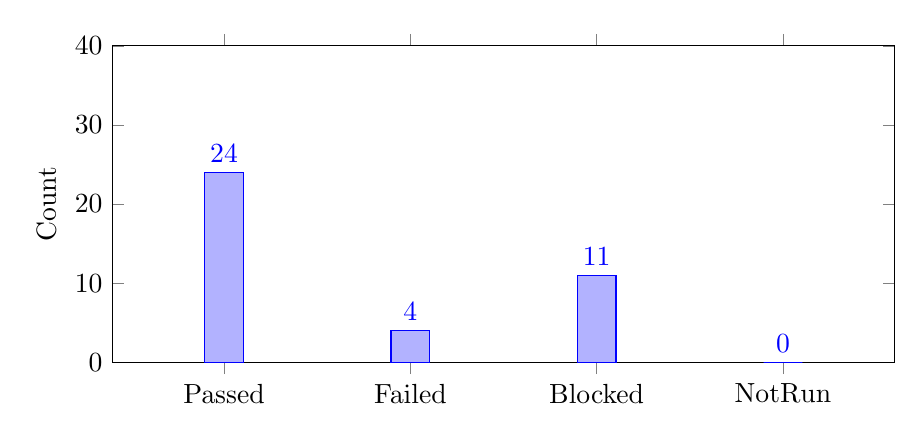
\begin{tikzpicture}
\begin{axis}[
  ybar,
  width=0.95\linewidth,
  height=5.6cm,
  bar width=14pt,
  ymin=0,
  ymax=40,
  ylabel={Count},
  symbolic x coords={Passed,Failed,Blocked,NotRun},
  xtick=data,
  nodes near coords,
  nodes near coords align={vertical},
  every axis plot/.append style={fill=blue!55},
  enlarge x limits=0.20
]
\addplot coordinates {(Passed,24) (Failed,4) (Blocked,11) (NotRun,0)};
\end{axis}
\end{tikzpicture}
\caption{Current manual test status derived from the VisionEdge device test report.}
\label{fig:teststatus}
\end{figure}

\subsection{Module-Wise Test Distribution}
\begin{table}[!t]
\centering
\small
\begin{tabular}{p{0.24\linewidth} c c c}
\toprule
Module & Passed & Failed & Blocked \\
\midrule
M1 Visual Perception & 4 & 1 & 1 \\
M2 Text Description & 4 & 0 & 1 \\
M3 Offline TTS & 2 & 0 & 3 \\
M4 Low Latency & 1 & 2 & 3 \\
M5 Accessibility \& Control & 4 & 0 & 1 \\
M6 Privacy \& Security & 1 & 1 & 1 \\
M7 User Interface & 5 & 0 & 0 \\
M8 Model Loading & 3 & 0 & 1 \\
\bottomrule
\end{tabular}
\caption{Current 39-case distribution summarized by test module.}
\label{tab:moduletestsummary}
\end{table}

\subsection{Representative Manual Cases}
\begin{table*}[t]
\centering
\begin{tabular}{p{0.08\linewidth} p{0.10\linewidth} p{0.16\linewidth} p{0.56\linewidth}}
\toprule
TC ID & Status & Category & Evidence \\
\midrule
TC-01 & Passed & Startup & Device UI and logs showed active preview startup with \texttt{Assistance ON} and \texttt{Live camera preview}. \\
TC-02 & Failed & Realtime capture & Throughput is still below target. Active-session UI showed only 12 captured frames with average latency near 1.7 s, so the formal 2 fps requirement is not yet met. \\
TC-03 & Passed & Detection & Repeated live detections were observed on hardware, including unknown-obstacle fallback and named object outputs. \\
TC-04 & Passed & Permissions & Missing camera permission routes to a dedicated onboarding permission gate with \texttt{Grant Camera Access}. \\
TC-12 & Passed & Offline TTS & Device logs confirmed local voice initialization, queueing, playback, and completion. \\
TC-17 & Passed & Latency & The live UI reported end-to-end latency of \texttt{1547 ms}; the stopped-session summary retained \texttt{1766 ms}, both within the 2 s requirement. \\
TC-21 & Failed & Memory & \texttt{dumpsys meminfo} reported \texttt{TOTAL PSS: 631210 KB} during an active session, above the 200 MB target. \\
TC-23 & Passed & User control & Single-tap start assistance path and spoken confirmation were observed on device. \\
TC-28 & Blocked & Privacy/network & In Expo dev-client mode, Metro/bootstrap traffic exists by design, so the formal no-network case cannot be judged from this environment. \\
TC-29 & Failed & Privacy/storage & \texttt{run-as} storage audit still found transient \texttt{cache/visionedge-captures/*.jpg} files while assistance was active. \\
TC-30 & Passed & Session cleanup & After stopping assistance, the transient capture directory was deleted and only static assets plus model cache remained. \\
TC-31 & Passed & UI & Home screen rendering was confirmed. \\
TC-34 & Passed & Error UX & The current app includes a dedicated \texttt{ErrorScreen} with recovery copy and a \texttt{Retry} button. \\
TC-36 & Passed & Model init & Vision model loaded at startup from cached local file. \\
TC-37 & Passed & TTS init & Android TTS initialized with 473 local voices. \\
TC-38 & Passed & Delegate & Android GPU delegate activation was reported in logs. \\
TC-39 & Blocked & Fault injection & Corrupted-model handling was not executed on the installed device in this pass. \\
\bottomrule
\end{tabular}
\caption{Representative manual cases from the current 39-case execution matrix. The full matrix is maintained in \texttt{docs/VisionEdge\_TestReport.md}.}
\label{tab:manualcases}
\end{table*}

\section{Physical Device Validation}
\subsection{Reference Device}
The latest physical validation run used:
\begin{itemize}[leftmargin=1.2em]
\item device: Nothing A001 (\texttt{GalagaIND}),
\item OS: Android 16,
\item connection: USB ADB,
\item package: \texttt{com.anonymous.visionedge}.
\end{itemize}

\subsection{Observed Runtime Evidence}
On the physical device, the following conditions were positively confirmed:
\begin{itemize}[leftmargin=1.2em]
\item Metro status endpoint on the host confirmed that the Metro bundler was running;
\item the ADB reverse tunnel reached device localhost after re-application;
\item the bundled model was cached to:
\begin{quote}
\codepath{file:///data/user/0/com.anonymous.visionedge/cache/models/yolo26s_float16.tflite}
\end{quote}
\item the TFLite runtime loaded the model with the Android GPU delegate in about 318 ms;
\item Android TTS reported 473 local voices;
\item the app reached the ``runtime is ready'' state without reproducing the earlier startup crash;
\item the realtime path still exposed a native crash in the resize/shared-buffer stage during assistance on the tested device;
\item app-private storage inspection found cached image artifacts that fail the current privacy/storage requirements.
\end{itemize}

\subsection{A Practical Engineering Finding}
One of the most important validation findings was operational, not algorithmic:
\begin{quote}
When the ADB daemon restarts, the \codeid{adb reverse tcp:8081 tcp:8081} tunnel can disappear. In that state, the dev build fails immediately with ``Unable to load script'' against \codeid{localhost:8081}, even though the app package itself is installed correctly.
\end{quote}

This finding is important because it distinguishes infrastructure failure from application failure. In the observed session, the device was able to reach Metro only after the reverse rule was re-applied and verified directly from the device shell.

\section{Results and Discussion}
\subsection{Verified Quantitative Evidence}
\begin{table}[!t]
\centering
\begin{tabular}{p{0.44\linewidth} p{0.33\linewidth}}
\toprule
Metric & Observed Value \\
\midrule
Bundled detector & YOLO26s TFLite \\
Input resolution & 320x320 \\
Vision model load time & 318 ms \\
TTS local voices & 473 \\
Automated suites passed & 9 / 9 \\
Automated tests passed & 33 / 33 \\
Manual cases passed & 24 / 39 \\
Manual cases failed & 4 / 39 \\
Manual cases blocked & 11 / 39 \\
Measured active latency & 1547 ms \\
Measured memory (PSS) & 631210 KB \\
\bottomrule
\end{tabular}
\caption{Current verified project measurements and counts.}
\label{tab:metrics}
\end{table}

\subsection{Interpretation}
These results support the following conclusions:
\begin{enumerate}[leftmargin=1.2em]
\item The project has successfully crossed the threshold from simulated local detection to a real bundled local detector.
\item The Android startup path is significantly healthier than earlier iterations because the model, delegate, and TTS stack now initialize reliably when Metro connectivity is correct.
\item The major remaining uncertainty is no longer model availability. It is the stability of the realtime native frame-processing path under live assistance.
\item The current system is strong enough to support continued optimization; it is not yet strong enough to claim complete validation of all SRS performance, privacy, and robustness requirements.
\end{enumerate}

\section{Screenshots and Visual Evidence}
The repository contains both UI mockup/reference screens and ADB captures from device testing.

\begin{figure*}[!t]
\centering
\begin{minipage}[t]{0.48\textwidth}
\centering
\imagebox{0.72}{../../screenshots/adb-intro-screen.png}
\caption{ADB-captured intro screen.}
\label{fig:adbintro}
\end{minipage}\hfill
\begin{minipage}[t]{0.48\textwidth}
\centering
\imagebox{0.72}{../../screenshots/adb-home-screen.png}
\caption{ADB-captured home screen.}
\label{fig:adbhome}
\end{minipage}
\end{figure*}

\begin{figure*}[!t]
\centering
\begin{minipage}[t]{0.31\textwidth}
\centering
\imagebox{0.78}{../../screenshots/main_screen.jpeg}
\caption{Main screen reference mockup from the repository.}
\label{fig:mainmock}
\end{minipage}\hfill
\begin{minipage}[t]{0.31\textwidth}
\centering
\imagebox{0.78}{../../screenshots/settings_sreen.jpeg}
\caption{Settings screen reference mockup from the repository.}
\label{fig:settingsmock}
\end{minipage}\hfill
\begin{minipage}[t]{0.31\textwidth}
\centering
\imagebox{0.78}{../../screenshots/debug_screen.jpeg}
\caption{Debug summary screen reference mockup from the repository.}
\label{fig:debugmock}
\end{minipage}
\end{figure*}

\section{Gap Analysis: Planned Design vs Current Reality}
\subsection{What Is Fully Aligned}
The current implementation is aligned with the original project vision in the following areas:
\begin{itemize}[leftmargin=1.2em]
\item offline-first design,
\item camera-to-detection-to-speech pipeline,
\item accessible user interaction,
\item local settings and session-state persistence,
\item emphasis on low-latency feedback,
\item no mandatory cloud dependency.
\end{itemize}

\subsection{What Changed in the Concrete Implementation}
The present implementation differs from the SDS in several practical ways:
\begin{itemize}[leftmargin=1.2em]
\item It uses React Native VisionCamera worklets instead of a generic mobile camera abstraction.
\item It uses Android system TTS rather than bundling a standalone neural TTS model.
\item It uses a YOLO26s TensorFlow Lite detector rather than an abstract ``compressed on-device vision model.''
\item It currently estimates distance heuristically from object box size rather than using a dedicated depth or monocular 3D model.
\end{itemize}

\subsection{What Is Still Incomplete}
The following items remain incomplete or only partially verified:
\begin{itemize}[leftmargin=1.2em]
\item stabilization of the native resize/shared-buffer path used during live assistance,
\item controlled foreground validation of live object detection and narration,
\item strict end-to-end latency measurement for REQ/PERF sign-off,
\item battery and memory profiling under sustained sessions,
\item closure of the currently failed and blocked cases in the 39-case validation suite,
\item stronger outdoor-road-specific semantic accuracy validation.
\end{itemize}

\section{Risk Assessment}
\begin{table}[!t]
\centering
\small
\begin{tabularx}{\linewidth}{>{\raggedright\arraybackslash}p{0.25\linewidth} >{\raggedright\arraybackslash}p{0.18\linewidth} >{\raggedright\arraybackslash}X}
\toprule
Risk & Current Severity & Mitigation \\
\midrule
Metro tunnel loss in dev build & High during development & Re-apply and verify \texttt{adb reverse}; document repeatable commands. \\
Foreground-device automation instability & Medium & Use ADB logs plus manual physical validation; do not over-claim screenshot evidence. \\
Native resize/shared-buffer crash during live assistance & High & Harden the VisionCamera resize path, reduce native buffer handling risk, and validate on the reference phone before claiming latency targets. \\
Heuristic distance estimates & Medium & Future integration of monocular depth / 3D detection. \\
Live latency variability across phones & High & Keep input resolution low, retain delegate fallback, and continue profiling on real hardware. \\
Temporary cached JPEG persistence & High & Explicitly delete transient camera/manipulator artifacts and re-run SEC-2 and SEC-3 storage audits. \\
Dependence on system TTS voice characteristics & Medium & Future optional bundled neural TTS if consistent voice and latency become critical. \\
\bottomrule
\end{tabularx}
\caption{Key technical and validation risks in the current project state.}
\label{tab:risk}
\end{table}

\section{Future Work}
The next practical improvements should be:
\begin{enumerate}[leftmargin=1.2em]
\item stabilize the live VisionCamera resize/shared-buffer path on the reference device;
\item complete foreground live-scene sign-off for blocked manual tests;
\item improve object-distance estimation with a dedicated monocular depth or 3D detection model;
\item validate true end-to-end narration latency with repeated measurements on the reference device;
\item eliminate cached frame/image persistence and re-run the privacy/security cases;
\item expand the detector or post-processing for better road/outdoor obstacle coverage;
\item evaluate whether a lightweight bundled neural TTS model can outperform Android system TTS while staying within device resource limits.
\end{enumerate}

\section{Conclusion}
VisionEdge is no longer only a planned assistive system described in SRS and SDS documents. It is now a functioning Android implementation with a real local detector, a real offline speech path, automated tests, and physical-device validation evidence. The strongest engineering achievement of the current version is not merely that it detects objects; it is that it does so through a mobile architecture designed to respect realtime and privacy constraints.

At the same time, the honest state of the project is mixed. Startup, local model loading, TTS initialization, and GPU delegate activation are verified. The complete live assistance experience under a stable foreground device session is improved but not yet fully signed off against the full manual test suite. For a software engineering report, this distinction matters. A credible project report should document not only what the system was intended to do and what code exists, but what has actually been verified.

By that standard, VisionEdge is a credible and technically grounded offline assistive-perception prototype with a clear path to further improvement in distance estimation, live-scene robustness, and comprehensive device validation.

\begin{thebibliography}{99}

\bibitem{tan2020efficientdet}
M. Tan, R. Pang, and Q. V. Le, ``EfficientDet: Scalable and Efficient Object Detection,'' in \textit{Proc. IEEE/CVF Conf. Comput. Vis. Pattern Recognit.}, 2020, pp. 10781--10790, doi: 10.1109/CVPR42600.2020.01079.

\bibitem{xiong2021mobiledets}
Y. Xiong \textit{et al.}, ``MobileDets: Searching for Object Detection Architectures for Mobile Accelerators,'' in \textit{Proc. IEEE/CVF Conf. Comput. Vis. Pattern Recognit.}, 2021, pp. 3825--3834.

\bibitem{ren2021fastspeech2}
Y. Ren \textit{et al.}, ``FastSpeech 2: Fast and High-Quality End-to-End Text to Speech,'' in \textit{Proc. ICLR}, 2021, arXiv:2006.04558.

\bibitem{mehta2024matchatts}
S. Mehta, R. Tu, J. Beskow, E. Sz\'ekely, and G. E. Henter, ``Matcha-TTS: A fast TTS architecture with conditional flow matching,'' in \textit{Proc. IEEE ICASSP}, 2024, arXiv:2309.03199.

\bibitem{dang2024livespeech}
T. Dang, D. Aponte, D. Tran, and K. Koishida, ``LiveSpeech: Low-Latency Zero-shot Text-to-Speech via Autoregressive Modeling of Audio Discrete Codes,'' in \textit{Proc. Interspeech}, 2024, pp. 3395--3399, doi: 10.21437/Interspeech.2024-1192.

\bibitem{guo2024flytts}
Y. Guo, Y. Lv, J. Dou, Y. Zhang, and Y. Wang, ``FLY-TTS: Fast, Lightweight and High-Quality End-to-End Text-to-Speech Synthesis,'' in \textit{Proc. Interspeech}, 2024, arXiv:2407.00753.

\bibitem{vecino2023lightweighttts}
B. T. Vecino \textit{et al.}, ``Lightweight End-to-end Text-to-Speech Synthesis for Low-Resource On-Device Applications,'' in \textit{Proc. 12th ISCA Speech Synthesis Workshop}, 2023, pp. 225--229, doi: 10.21437/SSW.2023-35.

\bibitem{zhao2024rtdetr}
Y. Zhao \textit{et al.}, ``DETRs Beat YOLOs on Real-Time Object Detection,'' in \textit{Proc. IEEE/CVF Conf. Comput. Vis. Pattern Recognit.}, 2024, pp. 16965--16974.

\bibitem{cheng2024yoloworld}
T. Cheng, L. Song, Y. Ge, W. Liu, X. Wang, and Y. Shan, ``YOLO-World: Real-Time Open-Vocabulary Object Detection,'' in \textit{Proc. IEEE/CVF Conf. Comput. Vis. Pattern Recognit.}, 2024, pp. 16901--16911, arXiv:2401.17270.

\bibitem{wang2024yolov10}
A. Wang \textit{et al.}, ``YOLOv10: Real-Time End-to-End Object Detection,'' 2024, arXiv:2405.14458.

\bibitem{li2024unimode}
Z. Li, X. Xu, S.-N. Lim, and H. Zhao, ``UniMODE: Unified Monocular 3D Object Detection,'' in \textit{Proc. IEEE/CVF Conf. Comput. Vis. Pattern Recognit.}, 2024, pp. 16561--16570.

\bibitem{alrazgan2021slr}
M. Al-Razgan \textit{et al.}, ``A Systematic Literature Review on the Usability of Mobile Applications for Visually Impaired Users,'' \textit{PeerJ Comput. Sci.}, vol. 7, e771, 2021, doi: 10.7717/peerj-cs.771.

\bibitem{islam2023environmentdescription}
R. B. Islam, S. Akhter, F. Iqbal, M. S. U. Rahman, and R. Khan, ``Deep Learning Based Object Detection and Surrounding Environment Description for Visually Impaired People,'' \textit{Heliyon}, vol. 9, no. 6, e16924, 2023, doi: 10.1016/j.heliyon.2023.e16924.

\bibitem{takizawa2017spotreminder}
H. Takizawa, K. Orita, M. Aoyagi, N. Ezaki, and S. Mizuno, ``A Spot Reminder System for the Visually Impaired Based on a Smartphone Camera,'' \textit{Sensors}, vol. 17, no. 2, 291, 2017, doi: 10.3390/s17020291.

\bibitem{lin2017guidingsystem}
B.-S. Lin, C.-C. Lee, and P.-Y. Chiang, ``Simple Smartphone-Based Guiding System for Visually Impaired People,'' \textit{Sensors}, vol. 17, no. 6, 1371, 2017, doi: 10.3390/s17061371.

\end{thebibliography}

\end{document}
